\section{Produktübersicht}
\setboolean{@twoside}{false}
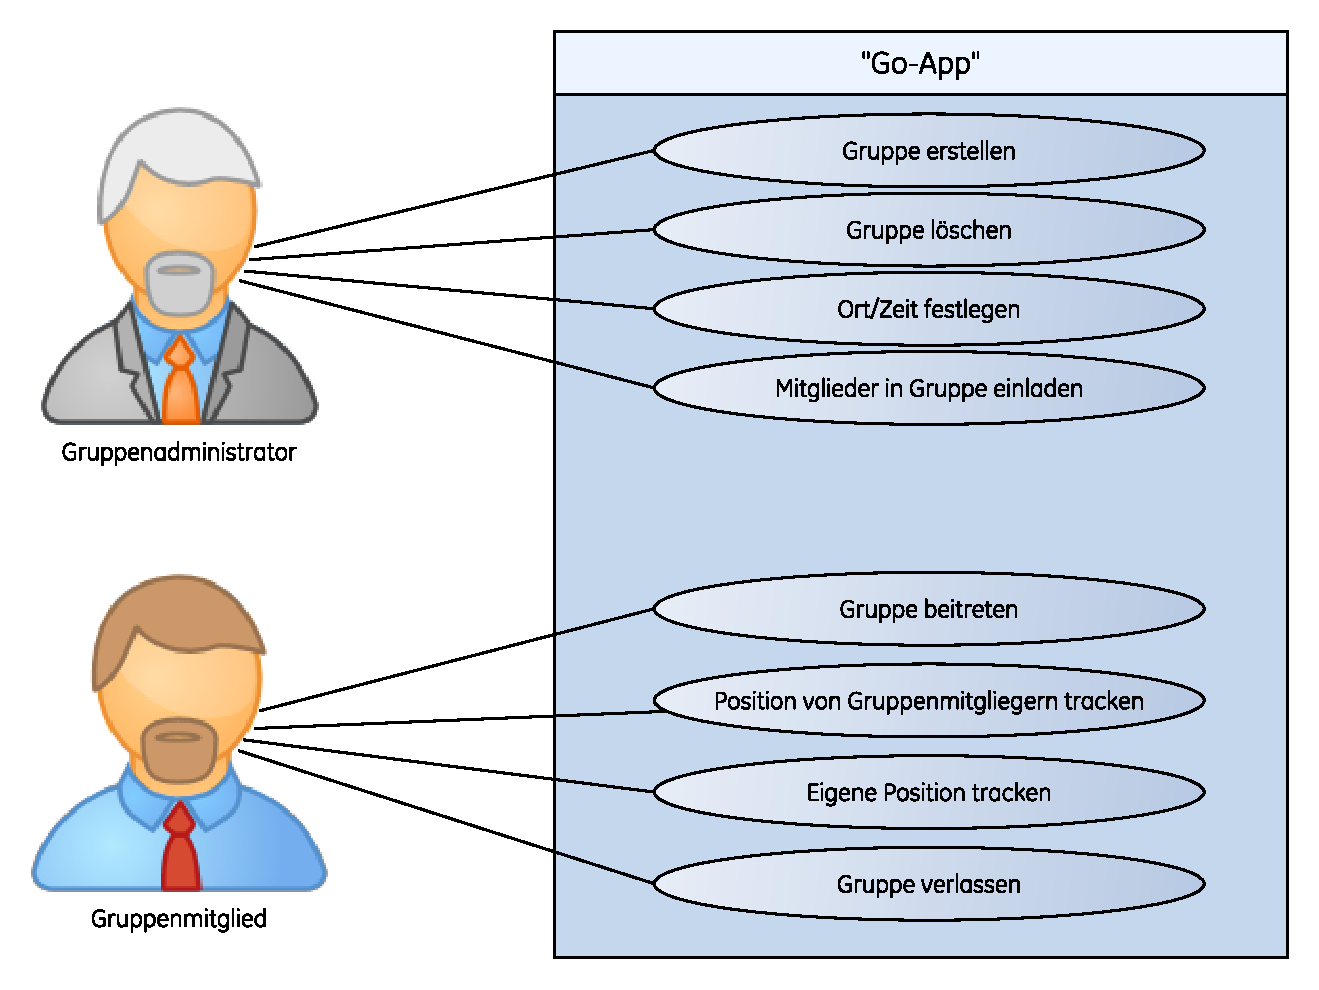
\includegraphics[scale=0.8, trim=2cm 0 0 0cm]{res/anwendungsfall.pdf}

\subsection{Systemarchitektur}

\begin{figure} [h]
	\centering
	\includegraphics[scale = 0.8]{res/clientServerArchitektur.png}
\end{figure}
Die Client-Server-Architektur wird verwendet, da mehrere Mobiltelefone nebeneinander ohne konkrete Kenntnis voneinander zu haben, Ressourcen des Servers anfragen. Dieser wertet die Anfrage aus und liefert eine Antwort zurück an den Client. \\
In unserem Fall steht jeder Benutzer über einen zentralen Server in Verbindung mit seinen Gruppen und kann so z.B. die Standorte der anderen Mitglieder anfragen und bekommt diese dann vom Server geliefert.

\subsection{Szenarien}
     Ein Benutzer erstellt eine neue Gruppe, da er sich gerne mit ein paar Freunden zu einem netten Abend treffen würde. Da er Gruppenadministrator und bisher außer ihm noch keiner in der Gruppe ist, lädt er über Mitglieder hinzufügen seine Freunde ein. Diese erhalten einen Link und werden automatisch zur Gruppe weitergeleitet und sind nun Mitglieder. \\
     Währenddessen hat der Gruppenadministrator schon den Zielort auf der Karte gesetzt und die Uhrzeit für den heutigen Abend eingetragen. Alle Mitglieder sehen nun, dass sie sich um 21:00 Uhr in Kneipe1 treffen. \\
     Um 20:55 Uhr drückt der Gruppenadministrator den Go-Button und macht sich auf den Weg zum Zielort. Auf der Karte sieht er nun, dass sich zwei seiner Freunde schon auf dem Weg befinden und nicht weit von ihm entfernt sind. Die zwei Freunde sehen umgekehrt natürlich auch den Gruppenadministrator und warten bis er zu ihnen aufgeschlossen hat. Gemeinsam laufen sie zu Kneipe1 und treffen dort die Anderen. Nach einer guten Stunde beschließt die Gruppe sich zu Kneipe2 aufzumachen, obwohl einer der Freunde noch immer nicht bei Kneipe1 angekommen ist. 
     Der Zielort wird nun also auf Kneipe2 und die Uhrzeit auf 22:30 Uhr gesetzt. \\
     Auch der letzte Freund macht sich auf den Weg und drückt den Go-Button. Er sieht, dass seine Freunde nun bei Kneipe 2 sind und diese sehen, dass er noch zu ihnen stoßen wird.
     Am Ende des Abends deaktivieren alle Mitglieder ihren Go-Button bzw. können sehen, ob jeder trotz hohem Alkoholpegel sicher nach Hause gekommen sind.
     
     
     
     %Eine Person erstellt eine neue Gruppe und ist damit Administrator, kurz: Admin.\\
     %Admin lädt Leute in die Gruppe ein via Share-Button. \\
     %Danach sucht er den Zielort über die Suchzeile. Als er ihn gefunden hat, platziert er die Nadel darüber.\\
     %Als nächstes setzt er den Zeitpunkt auf 21:00.\\
     %Person2 bekommt die Einladung in Form von Link über einen Messenger zugesendet.\\
     %Er tippt auf den Link und tritt der Gruppe bei. Er sieht den Zielpunkt und die Uhrzeit,\\
     %kann diese aber nicht ändern.\\
     %Um 20:55 drückt der Admin den Go-Button und macht sich auf den Weg zum Zielort.\\
     %Person2 sieht den Admin auf der Karte und dass er losgelaufen ist. Person2 drückt ebenfalls auf "GO" und läuft ebenfalls los.\\
     %Admin sieht, dass Person2 nur noch 100 Meter entfernt ist und wartet daher an einer geeigneten Stelle.\\
     %Admin und Person2 treffen sich schon vor dem Ziel und gehen gemeinsam weiter.\\
     %22:00: Der Admin setzt einen neuen Zielort "ClubX" und drückt den Go-Button.\\
     %Person2 ist in ein wichtiges Telefonat verwickelt. Deshalb bekommt er nicht mit,\\
     %dass der Admin schon weitergezogen ist.\\
     %Person2 ist fertig und sucht nach dem Admin. Er öffnet die App und sieht, \\
     %dass in der Gruppe ein neuer Zielort "ClubX" gesetzt wurde. Er sieht außerdem, dass der Admin bereits unterwegs ist.\\
     %Person2 drückt erneut den Go-Button um dem Admin zu signalisieren, dass er zurückgeblieben ist.\\
     %Danach macht er sich auf den Weg zum "ClubX" !!\\

Prof erstellt Gruppe und ist Admin\\
Prof lädt Mitarbeiter per link ein\\
Prof hält bis 13:00 Uhr Vorlesung und möchte danach in der Mensa essen gehen.\\
er setzt den Zeitpunkt auf 13:10 und den Standort auf „Mensa Adenauerring“\\
Kollegen und Mitarbeiter treten per link bei\\
13:00 Uhr, Prof drückt „Go“ und packt seine Sachen und geht los.\\
Kollegen bekommen notification dass Prof unterwegs ist.\\
Kollegen 1 - 5 machen sich sofort auf den Weg und drücken „Go“\\
Kollege 6 ist leider in einem Gespräch verwickelt\\
13:10 Prof und Kollegen treffen sich an der Mensa und gehen gemeinsam essen\\
13:15 Kollege 6 hat sein Gespräch beendet und bemerkt, dass sich seine Kollegen bereits in der Mensa befinden.\\
Kollege 6 drückt „Go“ und hastet zur Mensa\\
Kollege 6 trifft sich mit der Gruppe\\
Kollege 7 nimmt die Einladung zu spät an\\
er drückt dennoch auf „Go“ und geht los\\
Die Gruppe sieht, dass noch ein Nachzügler kommt und wartet auf 7\\

\subsection{Anwendungsfälle}
\subsubsection{Musskriterien}
\subsubsection{Wunschkriterien}
